\documentclass[11pt]{article}
\usepackage[czech]{babel}
\usepackage{ucs}
\usepackage[T1]{fontenc}
\usepackage[utf8]{inputenc}
\usepackage{amssymb}
\usepackage{graphicx}
\usepackage[paperheight=11cm, paperwidth=9cm, bottom=0.5cm, top=0.5cm, left=0.5cm, right=0.7cm]{geometry}



\emergencystretch=0pt
\pretolerance=150
\tolerance=250
\hbadness=150
\hfuzz=0pt
\emergencystretch=3em


\include{WordBreak.tex}


\begin{document}

\pagestyle{empty}

\section{Úvod}

Algebra je matematický obor, který se zabývá abstrakcí matematických objektů jako jsou například čísla, matematické operace a jiné. Dělí se do mnoha podskupin z nichž nejzákladnější je elementární algebra. Elementární algebra je nejzákladnější forma algebry, která navazuje na aritmetiku a zobecňuje aritmetické operace a jejich vlastnosti. Díky tomu lze tyto operace použít i na proměnné (prvky množin), nebo složitější matematické struktury. Hlavní rozdíl mezi aritmetikou a elementární algebrou je v použití proměnných. Díky tomu je možná abstraktní manipulace s čísly nebo dalšími operacemi, to je zobecnění dané vlastnosti na celou množinu.

Algebraické struktury jsou zobecněním aritmetických operací na množině {\it M}

Logická algebra je další důležitou oblastí algebry, protože má velké uplatnění ne jen v matematické logice, ale také v teorii logických obvodů a programování.

\subsection{Matematické objekty}

Matematický objekt je předmět zájmu matematického zkoumání, sloužící k výstavbě matematiky a její uplatnění v praxi. Nejzákladnějším příkladem matematického objektu je prvek množiny. Například libovolná čísla jsou matematické objekty, které se v aritmetice používají v aritmetických operacích. Jiný příklad matematického objektu jsou geometrické tvary, nebo matematické funkce nebo samotné množiny. Obecně lze říci, že se jedná o všechny fyzické objekty (podstatná jména) související s matematikou. Samozřejmě, že množinu nelze brát za fyzický předmět jako například dům, nebo že číslo 43 není fyzické jako nějaká osoba, ale používají se pro ně gramatické konstrukce jako pro fyzické objekty, na které si lze sáhnout.

\subsection{Proměnná}

Proměnná je v elementární algebře jeden z nejdůležitějších a nejzákladnějších objektů (pojmů). Proměnná je objekt, který v matematickém zápisu reprezentuje neurčitou hodnotu, může tedy vyjadřovat libovolný prvek (číslo) z dané množiny (většinou z množiny reálných čísel), která se nazývá {\bf obor proměnné}. Konkrétní čísla z oboru proměnné se nazývají {\bf hodnoty proměnné}. V matematických zápisech se proměnné většinou zapisuje pomocí znakového identifikátoru (jedineční znak, který danou proměnnou zastupuje) například {\it x, y, z, ...} Manipulace s proměnnými a vztahy pro ně platné mohou být chápány jako manipulace s libovolnými objekty, resp. vztahy platné pro všechny objekty (číselné hodnoty), které daná proměnná zastupuje.

\subsection{Konstanta}

Konstanta je opakem proměnné. Jedná se o pevně dané číslo (konkrétní prvek množiny), které má nějaký speciální význam pro danou aplikaci. Za konstantu je ale možné považovat i jakékoli jiné číslo, které nemá žádný speciální význam. Významné konstanty se zpravidla pojmenovávají pro jejich odlišení v matematických zápisech. Pro pojmenování významných konstant se používá slovní identifikátor a pro zkrácení zápisu ještě znakový identifikátor. Typickým příkladem může být číslo pí (3,14...), které se značí řeckým písmenem $\pi$ .

\subsection{Neznámá}

Neznámá je speciální případ proměnné. Jedná se o kombinaci proměnné a konstanty. Neznámou v zápise zastupuje znakový identifikátor, stejně jako v případě proměnné. Ale většinou není v danou chvíli její hodnota známa, ale může jí podle její definice zastupovat pouze jedna konkrétní hodnota. Zjištění hodnoty neznámé proměnné je cílem matematických výpočtů, respektive rovnic.

\section{Výrazy}

Výraz je každý matematický zápis, který je tvořen z konstant a proměnných, mezi nimiž jsou pomocí aritmetických operací sčítání, odčítání, násobení, dělení, mocnina a odmocnina a závorek vytvořeny smysluplné vztahy.

Algebraické výrazy lze rozdělit na několik druhů, podle charakteristických vlastností spjatých s operacemi, které obsahují. Algebraické výrazy v nichž se {\bf nevyskytují} odmocniny se nazývají {\bf racionální algebraické výrazy} (hodnotou racionálního výrazu může být vždy jen racionální číslo). Racionální výrazy se dále dělí na {\bf racionální celistvé výrazy} ({\it mnohočleny}) a {\bf racionální lomené výrazy}. Racionální celistvý výraz je výraz ve tvaru:

$$ (a \circ b) $$

Racionální lomený výraz je výraz ve kterém se nachází podíl, přičemž dělitelem je nenulový výraz, nebo proměnná (kdyby byla dělitelem konstanta, výraz by šel zkrátit a celý podíl by zmizel):

$$ {a \over b}$$

Algebraické výrazy ve kterých se nacházejí odmocniny se nazývají {\bf iracionální algebraické výrazy} (hodnotou iracionálního výrazu může být kromě racionálního čísla také iracionální číslo). Důležité je, že v odmocnině musí být proměnná výrazu, protože jinak by bylo možné odmocninu vyčíslit a nahradit konstantní hodnotou:

$$ \root n\of{a^m} $$

Dále se rozlišují {\bf goniometrické výrazy}, které obsahují alespoň jednu goniometrickou operaci nad danou proměnno, {exponenciální výraz}, ve kterém se nachází alespoň jedna proměnná v exponentu mocniny a {\bf logiaritmický výraz}, který obsahuje alespoň jedenu operaci logarimus nad danou proměnnou.


Pokud výraz lze rozložit na jednotlivé dílčí výrazy, nazývá se {\bf složený výraz}:

$$ (a \circ b) \bullet (a \circ b) \bullet ... \bullet (a \circ b) $$

Jednotlivé dílčí výrazy $(a \circ b)$ složeného výrazu se nazývají {\bf složky výrazu}.

Pokud se ve výrazu vyskytují pouze čísla, jedná se o {\bf aritmetický (konstantní) výraz}, protože jeho hodnota je vždy stejná (konstantní). Aritmetický výraz se značí pomocí velkého písmene, nejčastěji {\it V} od slova výraz, pojmenování může ale být libovolné a v nedůležitých zápisech se dokonce žádné pojmenování zpravidla nepoužívá:

$$ V = (5 + 3) $$

Pokud se ve výrazu vyskytuje alespoň jedna neznámá hodnota jedná se o {\bf algebraický výraz}, u kterého je nutné definovat podmínky za kterých má výraz smysl (definiční obor). Hodnota algebraického výrazu je závislá na hodnotě proměnné (popřípadě více proměnných), která se v něm vyskytuje. Algebraický výraz se značí podobně jako aritmetický, pomocí velkého písmene, ale následuje za ním ještě v závorce seznam proměnných, které se nacházejí v daném výrazu:

$$ V(a,b) = (ma + nb) $$

Čísla {\it m}, {\it n} určují podle vlastnosti operace součin, kolikrát se v daném výrazu nacházejí dané proměnné. Tato čísla se nazývají {\bf koeficienty proměnné výrazu}.

Složený výraz může být složen i z jiných pojmenovaných výrazů. {\bf Pojmenované výrazy} zastupují často používané a praxi důležité výrazy. Typickým příkladem jsou goniometrické výrazy sinus, cosinus, ... nebo logaritmust a jiné:

$$ V(x,y) = 2\cdot sin(x) + y $$

V případě  takového výrazu se stává seznam proměnných pojmenovaných výrazů součástí seznamu proměnných hlavního výrazu (seznam proměnných pojmenovaného výrazu je podmnožina seznamu proměnných hlavního výrazu). Proměnná, kterou pojmenovaný výraz ve svém těle používá se nazývá {\bf parametr výrazu}. 

Aby bylo možné s daným vnořeným výrazem dále pracovat, je nutné aby jeho vlastnosti v aritemtických operacích byly přesně definovány. Dále je nutné tyto vlastnosti zohlednit při budování definičních podmínek.

Algebraický výraz je základní pojem algebry, díky kterému je možné definovat pojmy rovnice, nerovnice, funkce, ... Jedná se o nástroje, které umožňují pracovat s výrazy pro jejich využití v praxy, a podrobně zkoumat jejich vlastnosti.

\subsection{Definiční obor výrazu}

{\bf Definiční obor výrazu} je množina hodnot, ze které je možné dosazovat konkrétní hodnoty za proměnné výrazu. Například množina reálných čísel, celých čísel, interval {\it (0:100)}, ... Pokud není předem určen definiční obor výrazu, je automaticky brán ten nejobecnější, tedy množina reálných čísel.

{\bf Definiční obor proměnné} je podmnožina definičního oboru výrazu ve kterém je více než jedna proměnná a je určen aritmetickou operací ve které se daná proměnná ve výrazu vyskytuje (respektive všemi operacemi ve kterých se daná proměnná vyskytuje).  V definičním oboru proměnné se nesmějí nacházet hodnoty, které nejsou pro danou aritmetickou operaci, ve které se nachází daná proměnná definovány. Jedná se tedy o jakousi pojistku, která zabrání zadávání neplatných hodnot do výrazu. Definiční obor výrazu slouží jako nosnou množina, ze které je vytvořen definiční obor proměnné.

\begin{center}
\scalebox{0.95}{ $ V(a,b,c) =( a \cdot {b \over c}) \rightarrow a, b \in R, c \in R \setminus \left\{0\right\} $}
\end{center}

Tento zápis vyjadřuje, že proměnné {\it a, b} jsou definovány na množině reálných čísel a proměnná {\it c} je definovaná na množině reálných čísel kromě nuly. Definiční obor výrazu definuje základní množinu ze které definiční podmínky vytvářející definiční obor pro jednotlivé proměnné definují, které proměnné je možné za danou proměnnou dosadit, aby výrazy s nimi dávaly smysl. Jako argument operace, ale může vystupovat i celý výraz a proto je potřeba vypočítat za jakých okolností (hodnot proměnných ve výrazu) může nabývat nepovolených hodnot pro danou operaci a tyto hodnoty pak vyjmout z definičního oboru výrazu.

Jestliže je ve výrazu {\it V} proměnných více $ V(x_1, x_2 , ... , x_n)$, pak jejich definiční obory tvoří uspořádanou množinu n-tic, jejíž prvky tvoří uspořádání hodnot, které mohou být dosazeny za jednotlivé hodnoty:

$$ (x_1, x_2, ... , x_n) \in \mathbb{R}^n $$

Hodnoty, které se nesmějí nacházet v definičním oboru proměnné jsou určeny pomocí {\bf definičních podmínek}, které říkají jakých hodnot daná proměnná nesmí nabývat. Příkladem může být nula ve jmenovateli zlomku, nebo záporná hodnota v sudé odmocnině:

$$ V(a, b) = a \circ b \rightarrow a \not = \left\{x, y, ... \right\}, b \not = \left\{ m, n, ...\right\} $$

\subsubsection{Určení definičních podmínek}

Definiční podmínky proměnné určují jaké hodnoty nesmějí být součástí definičního oboru dané proměnné. Tyto hodnoty vyplývají z aritmetických operacích, ve kterých se daná proměnná ve výrazu vyskytuje. Tyto hodnoty se dají buď odhadnout v případě, že se nejedná o složitý vztah a nebo je možné využít pokročilých matematických nástrojů jako jsou rovnice a nerovnice. 

Definiční podmínky je třeba řešit ne jen pro danou proměnnou, která se nachází ve výrazu s kritickou operací, ale je třeba pro celý výraz. Záleží totiž na hodnotě výrazu vstupující do operace. Hodnota výrazu je pak závislá na hodnotě proměnné, kterou daný výraz obsahuje.


\subsection{Obor hodnot výrazu}

Dosazením konstant za proměnné vznikne z algebraického výrazu výraz aritmetický, který lze jednoduše vyčíslit (vypočítat). {\bf Hodnotou výrazu} se rozumí výsledek získaný po dosazení daných hodnot z definičního oboru za všechny proměnné a provedení veškerých aritmetických operací (vyčíslení výrazu). Množina všech hodnot algebraického výrazu pro všechny hodnoty {\it x} z definičního oboru se nazývá {\bf obor hodnot}. Pro zjištění hodnoty daného výrazu je vždy třeba mít definované hodnoty, které mají být dosazeny za dané proměnné. Například po dosazení konstantní hodnoty {\it 3} do výrazu za proměnnou {\it x}:

$$ V(x) = (2x + 3) $$ 
$$ V(3) = 2\cdot 3 + 3 = 9 $$

{\bf Nulový bod výrazu} je taková hodnota, která po dosazení do výrazu vrátí po vyčíslení jeho nulu. Nulových bodů může být v závislosti na typu výrazu, respektive v závislosti na použitých aritmetických operacích více. V případě, že výraz obsahuje více než jednu proměnnou, tvoří nulový bod uspořádaná n-tice hodnot, která po dosazení za příslušné proměnné vrátí po vyčíslení výrazu nulu. Nulový bod daného výrazu se hledá pomocí rovnic. Příkladem je dosazení hodnoty {\it -2} do výrazu za proměnnou {\it x}:

$$ V(x) = (2x + 4)$$

$$ V(-2) = 2 \cdot (-2) +4 = -4 +4 = 0 $$

Za výraz lze dosadit třeba i jinou proměnnou, nebo pojmenovanou konstantu:

$$ V(x) = (2x + 4)$$
$$ V(y) = (2y + 4)$$

Výrazy se v matematických zápisech vyskytují velice často. Přehledný a snáze srozumitelný výraz totiž nahrazuje zdlouhavý slovní popis. Výrazy jsou také využívány ve formě vzorců a to ne jen v matematice, ale i v jiných vědních oborech jako je například fyzika a jiné.

\subsection{Rovnost algebraických výrazů}

Dva algebraické výrazy jsou si rovny:
$$ V_1 = V_2 $$

právě když pro ně platí:

\begin{itemize}
\item Výrazy mají společní definiční obor: $D(V_1) = D(V_2) = D$
\item Po dosazení libovolných stejných hodnot za proměnné do výrazu $V_1$ a $V_2$ jsou si hodnoty výrazů rovny: $V_1(x) = V_2(x)$
\end{itemize}


(Pozor! Nejedná se o rovnice, rovnice se rovnají pouze v určitých hodnotách výrazů při daných hodnotách x)


\subsection{Úpravy algebraických výrazů}

Podstatou úprav algebraidských výrazů je získat výraz nový v jednodušším tvaru, který je roven výrazu původnímu:

$$ V_1 \rightarrow V_2 \wedge V_1 = V_2 $$

Úprava algebraidských výrazů je důležitá pro získání minimálnícho (nejjednoduššího) tvaru výrazu. Díky tomu je práce s výrazy jednodušší a rychlejší. Úprava algebraického výrazu se řídí vlastnostmi aritmetických operací, které obsahuje.

Každý typ výrazu se upravuje specifickým způsobem podle vlastností algebraických (aritmetických) operací, které obsahuje.



\section{Mnohočleny}

Racionální celistvé výrazy tvoří členy ve tvaru $(ax + bx)$. Spojením více členů vznikají tzv. {\bf mnohočleny}. Podle definice racionálního celistvého výrazu může člen obsahovat neomezené množství proměnných a libovolnou přirozenou mocninou. Kdyby byl exponent mocniny záporný, dal by se výraz upravit na tvar zlomku s proměnnou ve jmenovateli $x^{-2} = {1\over x^{2}}$ a výraz by tak již nebyl racionální celistvý, ale racionální lomený. V případě, že by exponent proměnné byl reálný, dal by se výraz upravit na tvar s odmocninou $x^{1\over 2} = \sqrt{x}$ a výraz by tak byl iracionální.

{\bf Mnohočlen} nebo také {\bf polynom} je speciálním případem (tvarem) složeného výrazu, který obsahuje standardní aritmetické operace, konstanty a proměnné s n-tou mocninou. Platí, že každý mnohočlen je výraz, ale ne každý výraz je mnohočlen. Definice mnohočlenu zní - nechť je {\it n} přirozené číslo nebo nula, $ a_0, a_1, ..., a_n$ reálná čísla (konstanty) a {\it x} proměnná, pak součet:

$$ a_n \cdot x^n + a_{n-1} \cdot x^{n-1} + ... + a_1 \cdot x^1 + a_0 \cdot x^0  $$

se nazývá  mnohočlen (polynom) jedné {\bf proměnné x}, kde čísla $a_0, a_1, ..., a_n$ z oboru $\mathbb{R}$ se nazývají {\bf koeficienty mnohočlenu}. Dílčí výrazy $ (a_k \cdot x^k) $ pak se nazývají {\bf členy mnohočlenu}, kde číslo {\it k} definuje jejich stupeň. Charakteristickým rysem mnohočlenů je, že jsou jednotlivé členy (dílčí výrazy) navzájem sčítány. Číslo {\it n} se v zápisu nazývá {\bf stupeň mnohočlenu}. 

Je přípustné, aby některý z členů byl nulový: $a_n = 0$. V takovém případě dojde ke zrušení celé proměnné a členu výrazu: $(0 \cdot x^n) = 0$ a do zápisu mnohočlenu se tak vůbec nezapisuje. Tím se zpřehlední a zkrátí výsledný zápis. 

Stupeň mnohočlenu udává hodnotu nejvyššího exponentu, který se v mnohočlenu vyskytuje. Mnohočlen nultého stupně je tedy každé reálné číslo různé od nuly. Mnohočlen nultého stupně se nazývá {\bf absolutní člen}, mnohočlen prvního stupně se nazývá {\bf lineární}, mnohočlen druhého stupně se nazývá {\bf kvadratický}, mnohočlen třetího stupně se nazývá {\bf kubický} a mnohočlen vyššího stupně se obecně nazývá {\bf mnohočlen n-tého stupně}. Číslu nula se říká nulový mnohočlen - jeho stupeň se nedefinuje. 

Mnohočlen s jedním členem se nazývá {\bf jednočlen}, se dvěma členy {\bf dvojčlen}, se třemi členy {\bf trojčlen}, a mnohočlen s více než třemi členy se nazývá obecně {\bf n-člen}. Mezi jednočleny patří také čísla různá od nuly včetně. 

Mnohočleny lze uspořádat dvěma způsoby. {\bf Sestupně}, kdy směrem vpravo exponent klesá a {\bf vzestupně}, kdy směrem vpravo exponent roste. V aritmetických operacích s mnohočleny je nutné mít všechny mnohočleny uspořádány stejným způsobem, aby nedocházelo k nepřehledným a nečitelným zápisům ve kterých je těžké se vyznat.

Mnohočlen pak lze zobecnit na libovolný počet proměnných:

\begin{center}
\scalebox{0.8}{
$ a_{k}x^{m}y^{n}...z^{o} + a_{k-1}x^{m-1}y^{n-1}...z^{o-1} + ... + a_{0}x^{0}y^{0}...z^{0}  $}
\end{center}

kde $a_1, a_2, ... a_k$ z oboru $\mathbb{R}$ jsou koeficienty mnohočlenu a $x^{m}, y^{n}, ... z^{o}$ jsou proměnné mnohočlenu. V případě, že se v mnohočlenu nachází více proměnných, pak se jejich exponenty sčítají a stupeň mnohočlenu je dán největší hodnotou součtu všech mocnin daného členu: $s = m + n + ... + o$


Pokud se u proměnné s nejvyšším exponentem v daném mnohočlenu nachází koeficient o hodnotě 1, pak se takový mnohočlen nazývá {\bf normovaný}:

$$ 1\cdot x^5 + 2\cdot x +3$$


\subsection{Operace s mnohočleny}

S mnohočleny je možné vykonávat standardní operace součet, rozdíl, součin, podíl a umocnění na přirozený exponent. Při umocenění na reálný exponent by mohlo dojít k odmocňování mnohočlenu čímž by vzniknul iracionální výraz. 

\subsubsection{Rovnost mnohočlenů}
Dva mnohočleny se stejnými proměnnými jsou si {\bf rovny}, právě když se sobě rovnají všechny koeficienty odpovídajících si členů obou mnohočlenů (členů obsahující stejné mocniny proměnných). To vyplývá z obecné vlastnosti rovnosti algebraických výrazů. Jestliže jednotlivé členy tvoří dílčí algberaické výrazy, pak jsou si dva členy rovny právě tehdy, když mají stejný definiční obor a na něm stejný obor hodnot. To je možné pouze v případě, žeobsahují stejnou proměnnou, exponent a koeficient. 


\subsubsection{Součet a rozdíl mnohočlenů}

Součtem, popřípadě rozdílem výrazů je myšlen součet (rozdíl) hodnot koeficientů stejných proměnných, přičemž některé z koeficientů těchto mnohočlenů mohou být nulové:

$$ (2a+b) + (a+b) = 3a + 2b $$

Nelze sčítat dvě různé proměnné, protože obě reprezentují navzájem různé hodnoty z dané množiny čísel a jejich součtem vznikne neznámá hodnota se kterou nelze pracovat. Lze ale sčítat stejné proměnné a definovat tím kolik se jich ve výrazu vyskytuje, protože podle definice operace součin platí: $\underbrace{a+a+...+a}_n = n\cdot a$.

Rozdíl mnohočlenu se provádí jako součet prvního mnohočlenu a opačného mnohočlenu k druhému mnohočlenu. {\bf Opačný mnohočlen} k danému mnohočlenu je mnohočlen, který má tytéž členy, ale s opačnými znaménky:

$$ (3a+2b) - (a+b) = 3a + 2b + (-a -b) =  2a + b $$

{\bf Pozor na mínus před závorkou}. V případě, že se před závorkou nachází znaménko mínus, platí:$-(a+b)=-a-b$. Znaménko mínus funguje jako negující člen, čímž se hodnota proměnných a konstant uvnitř závorky invertuje na opačnou hodnotu (z kladné na zápornou a naopak).

\subsubsection{Součin mnohočlenu a proměnné (konstanty)}

Pro součin výrazu platí stejná pravidla jako pro aritmetický součin bez ohledu na to zda se jedná o proměnnou, nebo konstantu. Výraz se násobí proměnnou tak, že proměnná vynásobí každou proměnnou, nebo konstantu výrazu:

$$ (a + b) \cdot k = (k\cdot a) + (k \cdot b) $$

Toto pravidlo lze jednoduše odvodit z definice operace součin, protože platí, že $a \cdot b = \underbrace{b + b +.. +b}_a$ lze rozepsat součin výrazu a proměnné na:

\begin{center}
\scalebox{0.9}{
$ (a + b ) \cdot k = \underbrace{(a + b ) + (a + b ) +...+ (a + b )}_k$
}

\par
$=\underbrace{a + a + ... +a}_k + \underbrace{b + b +...+b}_k$
\par
$ = k\cdot a + k\cdot b $

\end{center}



\subsubsection{Součin dvou mnohočlenů}

Výraz se násobí výrazem tak, že každá proměnná, popřípadě konstanta jednoho výrazu násobí každou proměnnou, popřípadě konstantu druhého výrazu. Pokud se ve výsledném výrazu nacházejí dvě nebo více součinné tvary proměnných, popřípadě konstant, daný výraz je možné zkrátit jejich sečtením:

$$ (a \pm b) \cdot (c \pm d) = ac \pm ad \pm bc \pm bd $$

Podobně jako součin výrazu a proměnné lze rozepsat i součin dvou výrazů:

\begin{center}
\scalebox{0.9}{
$(a + b) \cdot (c + d) = \underbrace{(c + d) + (c + d) + ... + (c + d)}_{(a + b)} $}

$$ = \underbrace{c + c + ...+c}_{(a + b)} + \underbrace{d + d + ... +d }_{(a + b)} $$

\scalebox{0.7}{
$ = \underbrace{c + c ... +c}_{a} + \underbrace{c + c + ... +c}_{b} + \underbrace{d + d + ... +d}_{a} + \underbrace{d+d+...+d}_b $}

$$ = ac + ad + bc + bd $$
\end{center}

Protože každou hodnotu (proměnou) lze napsat jako: $a = a^1$, a zároveň při součinu mocnin se exponenty obou proměnných sčítají, platí, že součinem dvou stejných proměnných vznikne její druhá mocnina:

$$ a\cdot a = a^2 $$

Protože mnohočleny jsou zobecněním zápisu číselných hodnot, je možné s nimi provádět základní aritmetické operace - součet, rozdíl, součin, podíl, mocnina, odmocnina. To je rozšířeno i na ostatní typy algebraických výrazů. Tyto operace jsou využívány při zjednodušování a úpravě výrazů do minimálnějšího a jednoduššího tvaru.

\subsubsection{Podíl mnohočlenu proměnnou (konstantou)}

Podíl výrazu a proměnné znamená podělit každý člen výrazu danou proměnnou:

$$ (a_{n}x^{n}+...+a_0x^{0}) \div (ax^{k}) = {{a_nx^{n}}\over{ax^{k}}}+...+{{a_{0}x^{0}}\over{ax^{k}}} $$

To vyplývá z vlastnosti operace děleno, kterou lze převést na operaci násobení převedení na opačnou hodnotu pro danou aritmetickou operaci:
\begin{center}
\scalebox{0.7}{
$(a_{n}x^{n}+...+a_0x^{0}) \div (ax^{k}) = (a_{n}x^{n}+...+a_0x^{0}) \cdot ({{1} \over {ax^{k}}}) = ...  $}
\end{center}
\subsubsection{Podíl mnohočlenu mnohočlenem}

Podíl výrazu lze zobecnit na podíl libovlných dvou výrazů. Podmínkou je, aby obsahovaly stejné proměnné.

\subsubsection{Umocnění výrazu na n-tou}

Umocnit výraz na n-tou, kde číslo {\it n} je přirozené číslo, znamená podle definice mocniny znásobit vzájemně n-krát jeden výraz. Speciálním případem je umocnění výrazu na druhou mocninu, který je často používán. Jedná se o obecný vzorec rozkladu kvadratického dvojčlenu:


$$ (a + b)^2 = (a + b) \cdot (a + b) $$

$$=a^2 + ab + ab + b^2 = a^2 +2ab +b^2 $$


$$ =(a-b)^2 = (a-b) \cdot (a-b) $$

$$= a^2 -ab -ab +b^2 = a^2 -2ab + b^2 $$

$$ = a^2-b^2 = (a + b) \cdot (a-b) $$

Na důkaz této rovnosti je třeba použít opačný postup:

$$ (a + b) \cdot (a-b) = a^2 -ab +ab -b^2 = a^2-b^2 $$

Zobecnění umocnění výrazu na n-tou podrobně řeší {\bf Binomická věta}.

\subsection{Rozklad mnohočlenu na součin}

Rozlkadem mnohočlenu je myšleno jeho vyjádření jako součin jednodušších dále nerozložitelných mnohočlenů. K tomu lze využít několik postupů. Pomocí rozkladu na součin je v mnoha případech možné jednodušeji najít hodnoty nulových bodů daného mnohočlenu - jestliže je v součinu jeden člen roven nule, je roven nule celý mnohočlen. Kromě toho je díky rozkladu mnohočlenu možné výrazně zjednodušit zápis daného mnohočlenu, nebo zjednodušit operaci s mnohočleny.

\subsubsection{Rozklad pomocí vytýkání před závorku}

Vytýkání výrazu (mnohočlenu) před závorku je opačným postupem k násobení výrazů (roznásobení závorek). Jedná se o jednoduchou a přehlednou metodu jakou lze výraz rozložit na součin. 

Podstatou vytýkání je v každém z vytýkaných členu najít nějaký společný člen. To znamená, že vytýkané členy musejí být vzájemně soudělné - jedná se o násobky základního členu, který je použit pro vytýkání:

$$ ax + by = c\cdot (mx + ny) \Leftrightarrow a = m\cdot c \wedge b = n\cdot c $$

\subsubsection{Rozklad mnohočlenů pomocí vzorců}

Pro rozklad mnohočlenů na součin pomocí vzorců pro n-tou mocninu. Tyto vzorce lze použít pouze pro rozklad mnohočlenů s více proměnnými, ale pouze v určitém tvaru s mocninou.

Nejčastěji používané vzorce pro rozklad mnohočlenů jsou:

$$ a^2 -b^2 = (a-b)^2 \cdot (a+b)^2 $$
$$ a^3 - b^3 = (a-b) \cdot (a^2 + ab +b^2) $$
$$ a^3 + b^3 =(a+b)(a^2-ab+b^2) $$


Při rozkladu je je třeba nejprve třeba pomocí vlastností operace mocnina upravit daný mnohočlen na tvar odpovídající danému vzorci, který je vhodné použitít pro jeho rozklad.

\subsubsection{Doplnění na čtverec}
rozklad na čtverec


\subsection{Rozklad na kořenové činitele}



\section{Racionální lomenné výrazy}

\section{Iracionální výrazy}

\section{Exponenciální výrazy}

\section{Logaritmické výrazy}

\section{Goniometrické výrazy}

\section{Rovnice}

Rovnice jsou důležitým nástrojem matematiky, který umožňují určit, za jakých okolností (při jaké hodnotě proměnné proměnné, nebo více proměnných) jsou si hodnoty dvou různých výrazů rovny a zda si jsou vůbec někdy rovny, přičemž jeden z výrazů (pravá nebo levá strana rovnice) může být i konstantní (konstanta). To má velké uplatnění ve všech oborech, především technických. Tyto dva výrazy vyjadřují reprezentují reálné situace, které jsou v určitém vztahu (nebo nejsou v případě, že si v celém definičním oboru nejsou rovny). Typický příklad je postup zjištění jakou hodnotu (délku) musí mít strana čtverce, aby jeho obsah byl roven hodnotě {\it y} . Tímto způsobem je definováno (formulováno) mnoho fyzikálních a technických (a jiných) úloh. 

Jsou dány dva výrazy $L(x)$ a $P(x)$ proměnné {\it x} s definičním oborem {\it M}. Zápis 

$$ L(x) = P(x) $$

se nazývá {\bf rovnice} a vyjadřuje rovnost hodnot dvou výrazů v při dané hodnotě (hodnotách) proměnné {\it x}. Výrazu $L(x)$ se říká {\bf levá strana rovnice} a výrazu $P(x)$ se říká {\bf pravá strana rovnice}. Speciálním případem rovnice je rovnice, která má na jedné straně konstantu. Je-li touto konstantou nula, jedná se o {\bf anulovaný tvar rovnice}. Proměnná {\it x} se v kontextu rovnic nazývá neznámá {\bf neznámá} a k jejímu označení se zpravidla používají písmena z konce abecedy.

Po zadání konkrétních hodnot za proměnnou a vyčíslení výrazu na levé i pravé straně vznikně určitá konstantní hodnota. Řešení rovnice znamená najít množinu všech kořenů rovnice. Hodnoty neznámé $x_k$ pro které po vyčíslení platí rovnost výrazů $L(x) = P(x)$ se nazývají {\bf kořeny (řešení) rovnice}.

Číselný obor ($\mathbb{Z},\mathbb{R},\mathbb{C}, ...$) ve kterém se hledají kořeny rovnice se nazývá {\bf obor řešení rovnice}. Podmnožina množiny {\bf M} v níž jsou oba výrazy $L(x)$ a $P(x)$ definovány se nazývá {\bf definiční obor rovnice} (definiční podmínky výrazů). Množina hodnot, které představují kořeny rovnice se nazývá množina {\bf množina kořenů rovnice} a značí se písmenem {\bf K}. Platí:

$$ K \subseteq D \subseteq M $$

Pojem řešení rovnice se používá v několika případech:

\begin{itemize}
\item Pro kořen rovnice
\item Pro množinu kořenů rovnice
\item Pro postup jímž se určují kořeny rovnice
\end{itemize}

Konkrétní význam je buď zadán a nebo vyplývá ze situace.

\subsection{Rovnice s parametry}

Kromě známých mohou rovnice obsahovat další proměnné, jimž se říká {\bf parametry}. Značí se malými písmeny ze začátku abecedy, například {\it a}, {\it b}, {\it p}, … Taková rovnice se pak nazývá {\bf rovnice s parametry} a nebo  {\bf parametrická rovnice}. Parametrická rovnice představuje množinu všech rovnic, které se získají dosazením konstantních hodnot z dané číselné množiny (oboru parametru) za každý z parametrů.

Příkladem rovnice s parametry je: $ax = b$ s neznámou {\it x} a parametry $a, b \in \mathbb{R}$. Řešit rovnici s parametry znamená určit její kořeny v závislosti na přípustných hodnotách parametrů.

\begin{center}
\subsection{Grafický význam rovnic}
\end{center}


Význam rovnic a jejich řešení je dobře patrný z jejich grafického vyjádření. Pokud jsou výrazy na pravé a levé straně rovnice brány jako funkce, pak je možné z definičního oboru funkce a oboru hodnot obou výrazu vytvořit grafy v kartézské soustavě souřadnic, který přesně vypovídá při jakých hodnotách jsou si oba výrazy (funkce) rovny. Grafy obou výrazu se budou protínat právě v místech, kde má daná rovnice řešení. 

\vskip 4mm
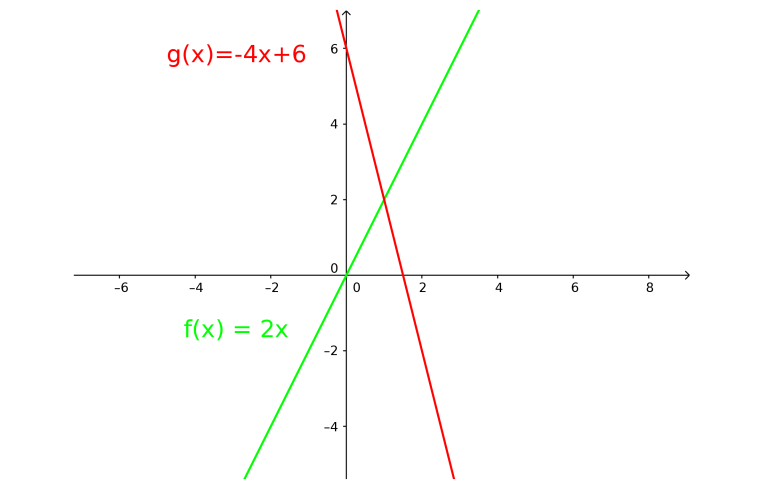
\includegraphics[width=\linewidth]{Obrazky/GrafickeReseniRovnic.png}
\vskip 4mm

První souřadnice je hodnota proměnné x,

Z grafické interpretace rovnic lze usoudit, kolik různých řešení může rovnice mít. Lze tak snadno zodpovědět otázky jako: má daná rovnice řešení? Může mít rovnice více než jedno řešení? Může mít rovnice nekonečně mnoho řešení? 

\subsection{Části postupu řešení rovnic}

\subsection{Klasifikace rovnic}

V základu se rovnice dělí na dvě skupiny:

\begin{itemize}
\item Algebraické (polynomické) rovnice
\item Nealgebraické (transcendentní) rovnice
\end{itemize}


{\bf Alegebraické rovnice} n-tého stupně s neznámou $x \in \mathbb{R}$ je každá rovnice ve tvaru:

$$ a_nx^n + a_{n-1}x^{n-1} + ... + a_1x + a_0 = 0 $$

kde $a_0$, $a_1$, ... $a_n$ jsou reálná čísla, která se nazývají {\bf koeficienty algebraické rovnice}.

Příkladem algebraických rovnic jsou lineární rovnice, kvadratické rovnice, ...

{\bf Nealgebraická rovnice} je každá rovnice, která není algebraická. Jsou to rovnice, které nemohou být vyjádřeny pomocí algebraických výrazů a aritmetických operací. Jedná se například iracionální rovnice, logaritmické rovnice, goniometrické rovnice, ... 

\subsection{Úpravy rovnic}


\section{Nerovnice}


\section{Soustavy rovnice}



\section{Soustavy nerovnic}


\end{document}
